\documentclass[12pt]{beamer}
\newenvironment{ConCodigo}[1]
  {\begin{frame}[fragile,environment=ConCodigo]{#1}}
  {\end{frame}}
\graphicspath{{Imagenes/}{../Imagenes/}}
\usepackage[utf8]{inputenc}
\usepackage[spanish]{babel}
\usepackage{hyperref}
\usepackage{etex}
\reserveinserts{28}
\usepackage{amsmath}
\usepackage{amsthm}
\usepackage{mathtools}
\usepackage{multicol}
\usepackage{multirow}
\usepackage{tabulary}
%\usepackage{tabularx}
\usepackage{booktabs}
\usepackage{nccmath}
\usepackage{biblatex}
\usepackage{epstopdf}
\usepackage{graphicx}
\usepackage{siunitx}
\sisetup{scientific-notation=true}
%\usepackage{fontspec}
\usepackage{lmodern}
\usepackage{float}
\usepackage[format=hang, font=footnotesize, labelformat=parens]{caption}
\usepackage[autostyle,spanish=mexican]{csquotes}
\usepackage{standalone}
\usepackage{tikz}
\usepackage[siunitx]{circuitikz}
\usetikzlibrary{arrows,patterns,shapes}
\usetikzlibrary{decorations.markings}
\usetikzlibrary{arrows}
\usepackage{color}
%\usepackage{beton}
%\usepackage{euler}
%\usepackage[T1]{fontenc}
\usepackage[sfdefault]{roboto}  %% Option 'sfdefault' only if the base font of the document is to be sans serif
\usepackage[T1]{fontenc}
\renewcommand*\familydefault{\sfdefault}
\DeclareGraphicsExtensions{.pdf,.png,.jpg}
\usepackage{hyperref}
\renewcommand {\arraystretch}{1.5}
\newcommand{\python}{\texttt{python}}
\usefonttheme[onlymath]{serif}
\setbeamertemplate{navigation symbols}{}
\usetikzlibrary{patterns}
\usetikzlibrary{decorations.markings}
\tikzstyle{every picture}+=[remember picture,baseline]
%\tikzstyle{every node}+=[inner sep=0pt,anchor=base,
%minimum width=2.2cm,align=center,text depth=.15ex,outer sep=1.5pt]
%\tikzstyle{every path}+=[thick, rounded corners]
\setbeamertemplate{caption}[numbered]
\newcommand{\ptm}{\fontfamily{ptm}\selectfont}
%Se usa la plantilla Warsaw modificada con spruce
\mode<presentation>
{
  \usetheme{Warsaw}
  \setbeamertemplate{headline}{}
  \useoutertheme{default}
  \usecolortheme{beaver}
  \setbeamercovered{invisible}
}
\AtBeginSection[]
{
\begin{frame}<beamer>{Contenido}
\normalfont\mdseries
\tableofcontents[currentsection]
\end{frame}
}

\usepackage{listings}
\lstset{ %
language=Python,                % choose the language of the code
basicstyle=\small,       % the size of the fonts that are used for the code
numbers=left,                   % where to put the line-numbers
numberstyle=\small,      % the size of the fonts that are used for the line-numbers
stepnumber=1,                   % the step between two line-numbers. If it is 1 each line will be numbered
numbersep=5pt,                  % how far the line-numbers are from the code
backgroundcolor=\color{white},  % choose the background color. You must add \usepackage{color}
showspaces=false,               % show spaces adding particular underscores
showstringspaces=false,         % underline spaces within strings
showtabs=false,                 % show tabs within strings adding particular underscores
frame=single,   		% adds a frame around the code
tabsize=2,  		% sets default tabsize to 2 spaces
captionpos=b,   		% sets the caption-position to bottom
breaklines=true,    	% sets automatic line breaking
breakatwhitespace=false,    % sets if automatic breaks should only happen at whitespace
escapeinside={\%},          % if you want to add a comment within your code
stringstyle =\color{magenta},
keywordstyle = \color{blue},
commentstyle = \color{green},
identifierstyle = \color{red}
}
\usepackage{siunitx}
\usepackage[american,cuteinductors,smartlabels]{circuitikz}
\usetikzlibrary{calc}
\title{Ecuaciones diferenciales ordinarias 2}
\subtitle{Curso de F\'{i}sica Computacional}
\author{M. en C. Gustavo Contreras May\'{e}n}
\begin{document}
\maketitle
\fontsize{14}{14}\selectfont
\spanishdecimal{.}
\begin{frame}{Contenido}
\tableofcontents[pausesections]
\end{frame}
\section{RK2 en EDO de orden superior}
\begin{frame}
\frametitle{RK2 para EDO de orden mayor}
Para utilizar el m\'{e}todo RK2 en una ecuaci\'{o}n diferencial de orden superior, veamos que es f\'{a}cil de aplicar. Sea una EDO de segundo orden del tipo:
\[ y''(t) +ay'(t) + by(t) = q(t), \]
\[y(0)=1, y'(0)= 0 \]
Donde $a$ y $b$ son coeficientes y $q(t)$ es una funci\'{o}n conocida, as\'{i} como las condiciones iniciales. Sea:
\[z(t) = y'(t)\]
\end{frame}
\begin{frame}
La ecuaci\'{o}n anterior se reduce a un sistema de EDO de primer orden:
\begin{eqnarray*}
y' = f(y,z,t) & \equiv & z \hspace{1cm} y(0) = 1 \\
z' = g(y,z,t) & \equiv & - az - by + q \hspace{1cm} z(0) = 0
\end{eqnarray*}
\end{frame}
\subsection{M\'{e}todo RK2 en las ecuaciones resultantes}
\begin{frame}
\frametitle{Expresi\'{o}n can\'{o}nica 1}
\begin{eqnarray*}
	k_{1} & = & hf(y_{n}, z_{n}, t_{n}) = hz_{n} \\
	l_{1} & = & hg(y_{n}, z_{n}, t_{n}) = h(-az_{n} - by_{n} + q_{n}) \\
	k_{2} & = & hf(y_{n}+k_{1}, z_{n}+l_{1}, t_{n+1}) = h(z_{n}+l_{1}) \\
	l_{2} & = & hg(y_{n}+k_{1}, z_{n}+l_{1}, t_{n+1}) = \\
	& = & h(-a(z_{n}+l_{1}) - b(y_{n}+k_{1}) + q_{n+1})
\end{eqnarray*}
\end{frame}
\begin{frame}
\frametitle{Expresi\'{o}n can\'{o}nica 2}
\begin{eqnarray*}
	y_{n+1} & = & y_{n} + \dfrac{1}{2}[k_{1}+k_{2}] \\
	z_{n+1} & = & z_{n} + \dfrac{1}{2}[l_{1}+l_{2}]
\end{eqnarray*}
\end{frame}
\subsection{Ejemplo}
\begin{frame}
\frametitle{Ejemplo}
Una masa $M = 0.5$ kg se une al extremo inferior de un resorte sin masa. El extremo superior se fija a una pared en reposo. La masa experimenta una resistencia $R = -B dy/dt$ debida al aire, donde $B$ es una constante de amortiguamiento. La ecuaci\'{o}n de movimiento es:
\[ M \dfrac{d^{2}}{dt^{2}}y + B \dfrac{d}{dt}y + ky = 0 \hspace{1cm}y(0)=1,y'(0)=0 \]
donde $k=100$ $k/s^{2}$ y $B=10$ $k/s$
\end{frame}
\begin{frame}
\frametitle{Sistema masa-resorte}
\begin{center}
\begin{tikzpicture}
	\tikzstyle{spring}=[thick,decorate,decoration={zigzag,pre length=0.1cm,post
	  length=0.1cm,segment length=6}]
	\draw (0,0) rectangle (1,1);
	\draw (0.3,1) -- (0.3,1.2);
	\draw[spring] (0.3,1.2) -- (0.3,2.2);
	\draw (0.3,2.2) -- (0.3,2.4);
	\draw (0.7,1) -- (0.7,1.5);
	\draw (0.5,1.5) -- (0.9,1.5);
	\draw (0.5,1.5) -- (0.5,1.7);
	\draw (0.9,1.5) -- (0.9,1.7);
	\draw (0.6,1.6) --(0.8,1.6);
	\draw (0.7,1.6) -- (0.7,2.4);
	\draw [pattern=north east lines] (-1,2.4) rectangle (2,2.7);
	\draw (1,0) -- (1.9,0);
	\draw [->] (1.8,2.4) -- node [midway, right] {y} (1.8,0);
\end{tikzpicture}
\end{center}
\[ M \dfrac{d^{2}}{dt^{2}}y + B \dfrac{d}{dt}y + ky = 0 \hspace{1cm}y(0)=1,y'(0)=0 \]
donde $k=100$ $k/s^{2}$ y $B=10$ $k/s$
\end{frame}
\begin{frame}
\frametitle{Re-escribimos la ecuaci\'{o}n}
\begin{eqnarray*}
	y' & = & z \equiv f(y,z,t) \hspace{2.5cm} y(0)=1 \\
	z' & = & - \dfrac{B}{M} z - \dfrac{k}{M} y \equiv g(y,z,t) \hspace{1.5cm} z(0)=0
\end{eqnarray*}
Sea $a=B/M=20$, $b=k/M=200$ y $g=0$.
\\
\bigskip
\textbf{Problema: } Calcular $y(t)$ para $0 < t < 0.05$ s, con el esquema RK2  y $h=0.025$ 
\end{frame}
\begin{frame}
\frametitle{Para $n=1$, $t=0.025$ tenemos que:}
\begin{eqnarray*}
	k_{1} &=& hf(y_{0},z_{0},t_{0}) = hz_{0} = 0.025(0) = 0 \\
	\visible<2->{l_{1} &=& hg(y_{0},z_{0},t_{0}) = h(-20z_{0}-200y_{0}) =} \\
	\visible<3->{      &=& 0.025(-20(0)-200(1))=-5} \\
	\visible<4->{k_{2} &=& hf(y_{0}+k_{1}, z_{0}+l_{1},t_{0}) = h(z_{0}+l_{1}) =} \\
	\visible<5->{	  &=& 0.025(0-5)=-0.125} \\
	\visible<6->{l_{2} &=& hg(y_{0}+k_{1},z_{0}+l_{1},t_{0}) =} \\
	\visible<7->{	  &=& h[-20(z_{0}+l_{1})-200(y_{0}+k_{1})]} \\
	\visible<8->{	  &=& 0.025[-20(0-5)-200(1+0)]=-2.5}
\end{eqnarray*}
\end{frame}
\begin{frame}
\frametitle{}
\begin{eqnarray*}
	y_{1} & = & y_{0} + \dfrac{1}{2}(0-0.125)=0.9375  \\
	z_{1} & = & z_{0} + \dfrac{1}{2}(-5-2.5)=-3.75
\end{eqnarray*}
\end{frame}
\begin{frame}
\frametitle{Ahora para $n=2$, $t=0.05$ tenemos que:}
\begin{eqnarray*}
	k_{1} &=& hf(y_{1},z_{1},t_{1}) = hz_{1} = -0.09375 \\
	\visible<2->{l_{1} &=& hg(y_{1},z_{1},t_{1}) = h(-20z_{1}-200y_{1})} \\
	\visible<3->{	  &=& -2.8125} \\
	\visible<4->{k_{2} &=& hf(y_{1}+k_{1}, z_{1}+l_{1},t_{1} = h(z_{1}+l_{1}) =} \\
	\visible<5->{	  &=& 0.1640625} \\
	\visible<6->{l_{2} &=& hg(y_{1}+k_{1},z_{1}+l_{1},t_{1}) =} \\
	\visible<7->{	  &=& h[-20(z_{1}+l_{1})-200(y_{1}+k_{1})]} \\
	\visible<8->{	  &=& -0.9375}
\end{eqnarray*}
\end{frame}
\begin{frame}
\frametitle{}
\begin{eqnarray*}
	y_{2} & = & y_{1} + \dfrac{1}{2}(0.09375-0.1640625)=0.80859  \\
	z_{2} & = & z_{1} + \dfrac{1}{2}(-2.8125-0.9375)=-5.625
\end{eqnarray*}
\end{frame}
\begin{frame}
\frametitle{Segunda parte del problema}
\begin{enumerate}
\item Calcula $y(t)$ para $0<t<10$ mediante RK2 y con $h=0.001$
\item Repite el ejercicio, ahora con $B=0$
\end{enumerate}
Para cada uno de los incisos, genera una gr\'{a}fica que acompañe a tu respuesta.
\end{frame}
\begin{frame}[fragile]
\frametitle{Soluci\'{o}n gr\'{a}fica, Y vs t, $B=10$ }
\begin{figure}
	\centering
	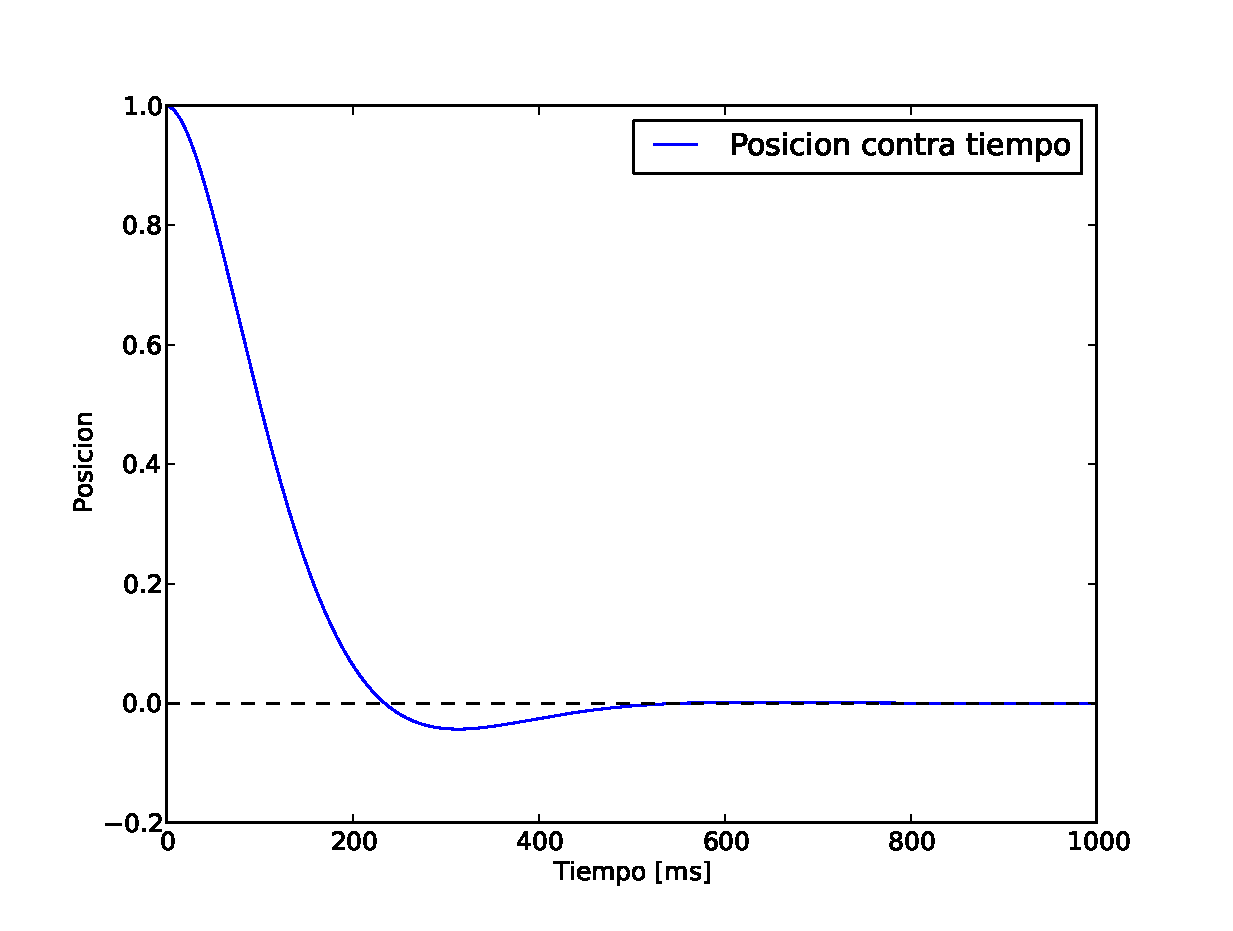
\includegraphics[scale=0.45]{RK2MasaResorte01.eps} 
\end{figure}
\end{frame}
\begin{frame}[fragile]
\frametitle{Soluci\'{o}n gr\'{a}fica, Z vs t, $B=10$}
\begin{figure}
	\centering
	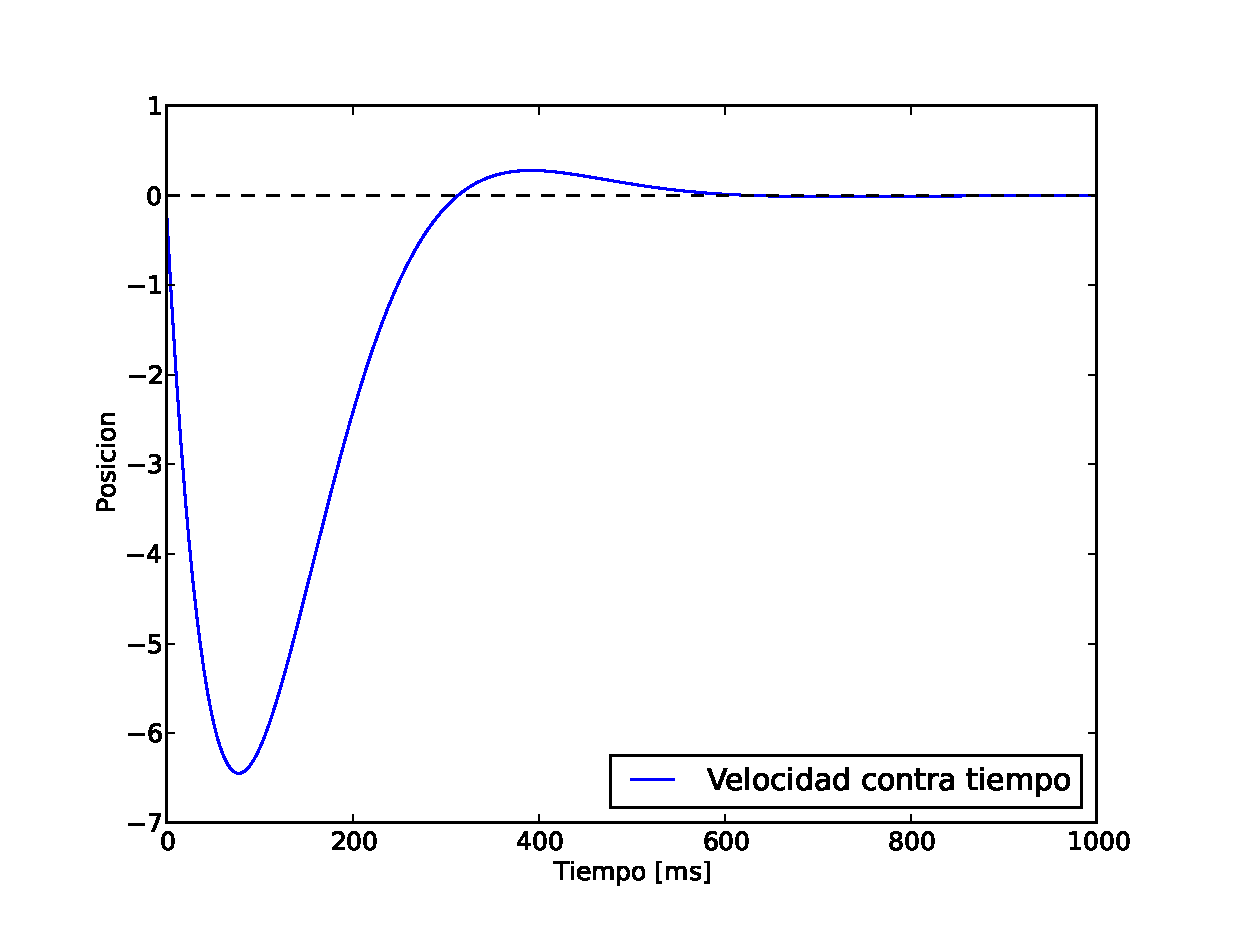
\includegraphics[scale=0.45]{RK2MasaResorte02.eps} 
\end{figure}
\end{frame}
\begin{frame}[fragile]
\frametitle{Soluci\'{o}n gr\'{a}fica, Y vs t, $B=0$ }
\begin{figure}
	\centering
	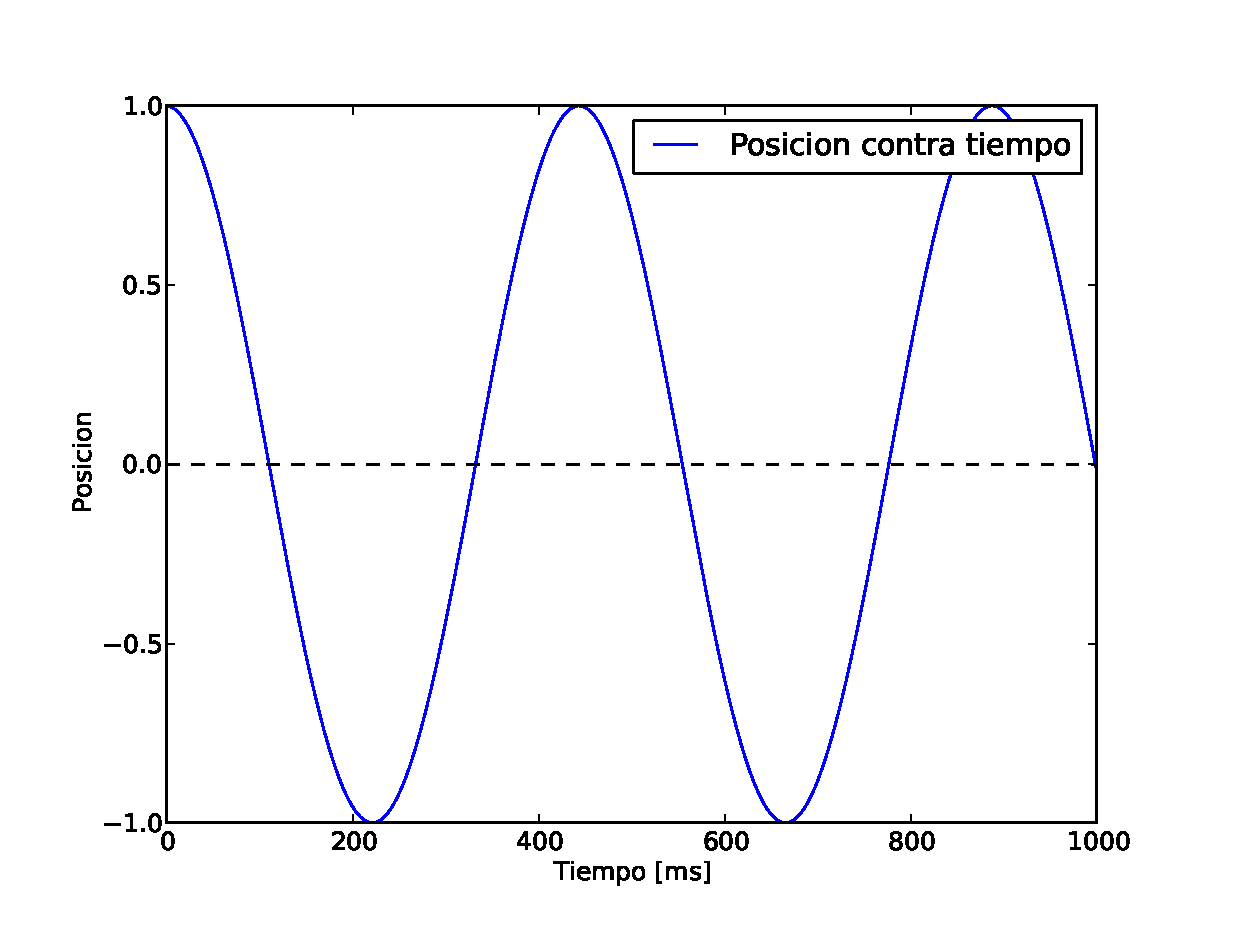
\includegraphics[scale=0.45]{RK2MasaResorte03.eps} 
\end{figure}
\end{frame}
\begin{frame}[fragile]
\frametitle{Soluci\'{o}n gr\'{a}fica, Z vs t, $B=0$}
\begin{figure}
	\centering
	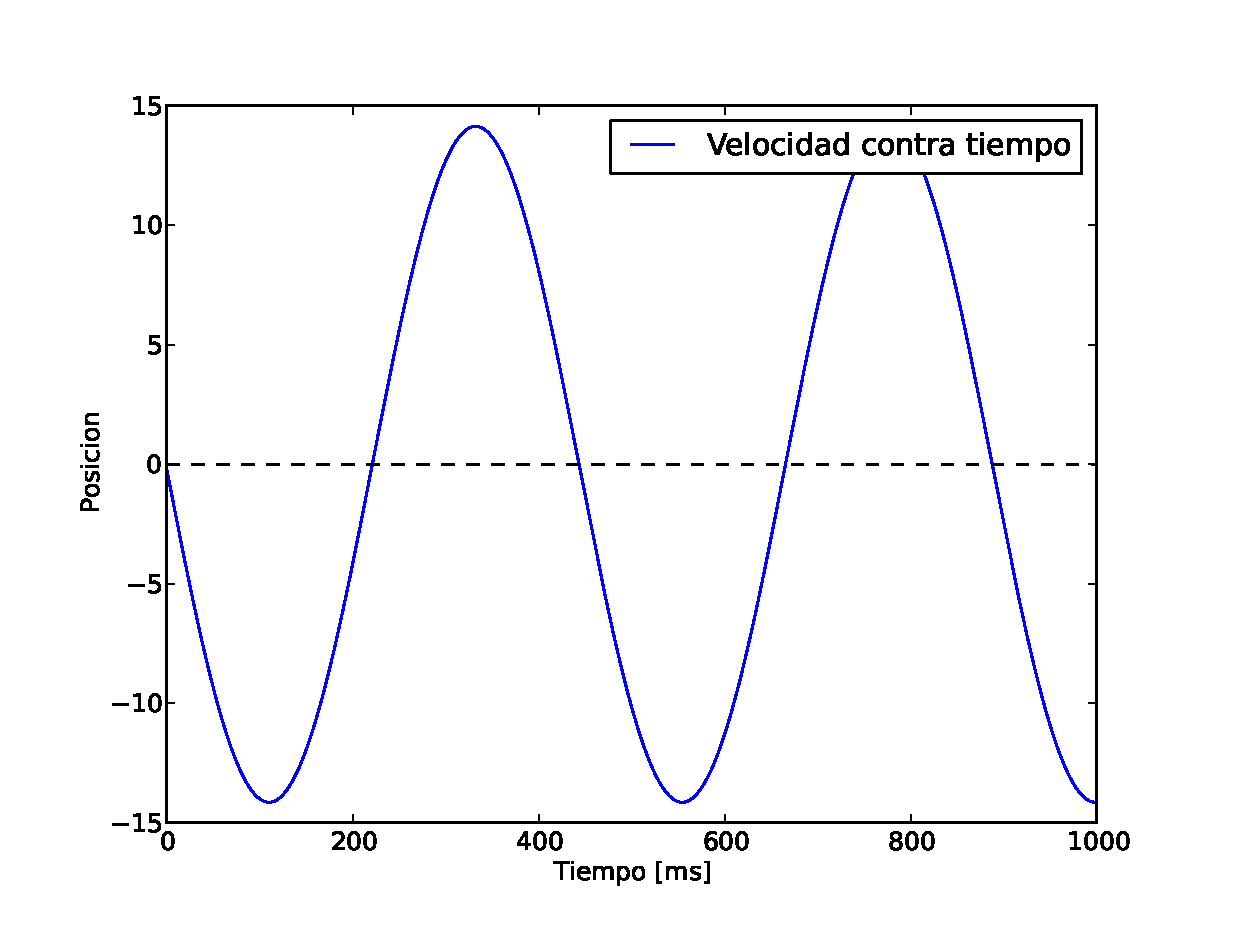
\includegraphics[scale=0.45]{RK2MasaResorte04.eps} 
\end{figure}
\end{frame}
\section{M\'{e}todo RK de tercer orden}
\begin{frame}
\frametitle{M\'{e}todo RK de tercer orden (RK3)}
Este m\'{e}todo es m\'{a}s preciso que el RK2. Se basa en la regla de 1/3 de Simpson, que como ya vimos en el tema anterior, se basa en la interpolaci\'{o}n polinomial cuadr\'{a}tica. El polinimio de Newton hacia adelante ajustado a $x_{0}$, $x_{1}$ y $x_{2}$ est\'{a} dado por la expresi\'{o}n:
\[ g(x_{0}+sh) = f_{0}+s(f_{1}-f_{0})+ \dfrac{s(s-1)}{2}(f_{2}-2f_{1}+f_{0}) \]
\end{frame}
\begin{frame}
Usando la regla de Simpson de 1/3 tenemos que:
\begin{equation*}
\begin{split}
	y_{n+1} = y_{n} +\dfrac{h}{6} [ f(y_{n},t_{n})+4f(y*_{n+\frac{1}{2}}, t_{n+\frac{1}{2}})+ \\
 +f(y*_{n+1},t_{n+1}) ]
\end{split}
\end{equation*}
Donde $y*_{n+1}$, $y*_{n+\frac{1}{2}}$ son estimaciones, puesto que no conocemos los valores de $y_{n+1}$, $y_{n+\frac{1}{2}}$
\end{frame}
\begin{frame}
Las estimaciones $y*_{n+1}$, $y*_{n+\frac{1}{2}}$ las desarrollamos con el m\'{e}todo de Euler hacia adelante:
\begin{eqnarray*}
	y*_{n+\frac{1}{2}} & = & y_{n} + \dfrac{h}{2} f(y_{n},t_{n}) \\
	y*_{n+1} & = & y_{n} + hf(y_{n},t_{n}) \hspace{0.5cm} \text{o bien}\\
	y*_{n+1} & = & y_{n} +h f(y*_{n+\frac{1}{2}},t_{n+\frac{1}{2}})
\end{eqnarray*}
\end{frame}
\begin{frame}
\frametitle{Expresi\'{o}n can\'{o}nica de RK3}
\begin{eqnarray*}
	k_{1} &=& hf(y_{n},t_{n}) \\
	k_{2} &=& hf(y_{n}+\dfrac{k_{1}}{2}, t_{n}+\dfrac{h}{2}) \\
	k_{3} &=& hf(y_{n}-k_{1}+2k_{2},t_{n}+h) \\
	y_{n+1} &=& y_{n}+\dfrac{1}{6}\left[k_{1}+4k_{2}+k_{3} \right] 
\end{eqnarray*}
\end{frame}
\section{M\'{e}todo de RK de cuarto orden (RK4)}
\begin{frame}
\frametitle{M\'{e}todo de Runge-Kutta de cuarto orden (RK4)}
El m\'{e}todo RK4 se obtiene de manera similar al de RK3, s\'{o}lo que se usa un paso intermedio adicional para evaluar la derivada.
\\
\medskip
El m\'{e}todo RK4 tiene una precisi\'{o}n hasta el t\'{e}rmino de cuarto orden del desarrollo de Taylor, por lo que el error local es proporcional a $h^{5}$
\end{frame}
\subsection{RK4 basado en la regla 1/3 de Simpson}
\begin{frame}
\frametitle{RK4 basado en la regla 1/3 de Simpson}
\begin{eqnarray*}
	k_{1} &=& hf(y_{n},t_{n}) \\
	k_{2} &=& hf(y_{n}+\dfrac{k_{1}}{2}, t_{n}+\dfrac{h}{2}) \\
	k_{3} &=& hf(y_{n}+\dfrac{k_{2}}{2},t_{n}+\dfrac{h}{2}) \\
	k_{4} &=& hf(y_{n}+k_{3}, t_{n}+h) \\
	y_{n+1} &=& y_{n}+\dfrac{1}{6}\left[k_{1}+2k_{2}+2k_{3}+k_{4} \right] 
\end{eqnarray*}
\end{frame}
\subsection{RK4 basado en la regla 3/8 de Simpson}
\begin{frame}
\frametitle{RK4 basado en la regla 3/8 de Simpson}
\begin{eqnarray*}
	k_{1} &=& hf(y_{n},t_{n}) \\
	k_{2} &=& hf(y_{n}+\dfrac{k_{1}}{3}, t_{n}+\dfrac{h}{3}) \\
	k_{3} &=& hf(y_{n}+\dfrac{k_{1}}{3}+\dfrac{k_{2}}{3},t_{n}+\dfrac{2h}{3}) \\
	k_{4} &=& hf(y_{n}+k_{1}-k_{2}+k_{3}, t_{n}+h) \\
	y_{n+1} &=& y_{n}+\dfrac{1}{8}\left[k_{1}+3k_{2}+3k_{3}+k_{4} \right] 
\end{eqnarray*}
\end{frame}
\section{Ejercicio}
\begin{frame}
\frametitle{Ejercicio}
Una pieza met\'{a}lica con una masa de $0.1$ kg a $200^{\circ}$ C  ($473$ K), se coloca en cierto momento en un cuarto cuya temperatura es $25^{\circ}$ C, en donde la pieza est\'{a} sujeta al proceso de enfriamiento por convecci\'{o}n natural y transferencia de calor por radiaci\'{o}n.
\end{frame}
\begin{frame}
Suponemos que la distribuci\'{o}n de temperatura es uniforme en la pieza, la ecuaci\'{o}n de T vs t es:
\[ \dfrac{dT}{dt} =  \dfrac{A}{(\rho c v)} [ \epsilon \sigma (297^{4} - T^{4})+ h_{c}(297-T)] \]
con $T(0)=473$ donde $T$ es la temperatura en grados Kelvin y las constantes son:
\end{frame}
\begin{frame}
\begin{tabular}{r l}
	$\rho =$  & 300 $\frac{k}{m^{3}}$ -- densidad del metal \\
	$v=$  & 0.001 $m^{3}$ -- volumen del metal \\
	$A=$ & 0.25 $m^{2}$ -- \'{a}rea de la superficie del metal \\
	$c=$ & 900 $\frac{J}{kK}$ -- calor espec\'{i}fico del metal \\
	$h_{c}=$ & 30 $\frac{J}{m^{2}K}$ coeficiente de transferencia de calor \\
	$\epsilon=$ & 0.8 -- emisividad del metal \\
	$\sigma=$ & 5.67 $\times 10^{-8}$ $\dfrac{w}{m^{2}K^{2}}$ cte Stefan-Boltzamann
\end{tabular}
Calcular el valor de T para el intervalo $0 < t < 300$ segundos, usa $h=0.25$
\end{frame}
\begin{frame}[fragile]
\frametitle{Soluci\'{o}n gr\'{a}fica}
\begin{figure}
	\centering
	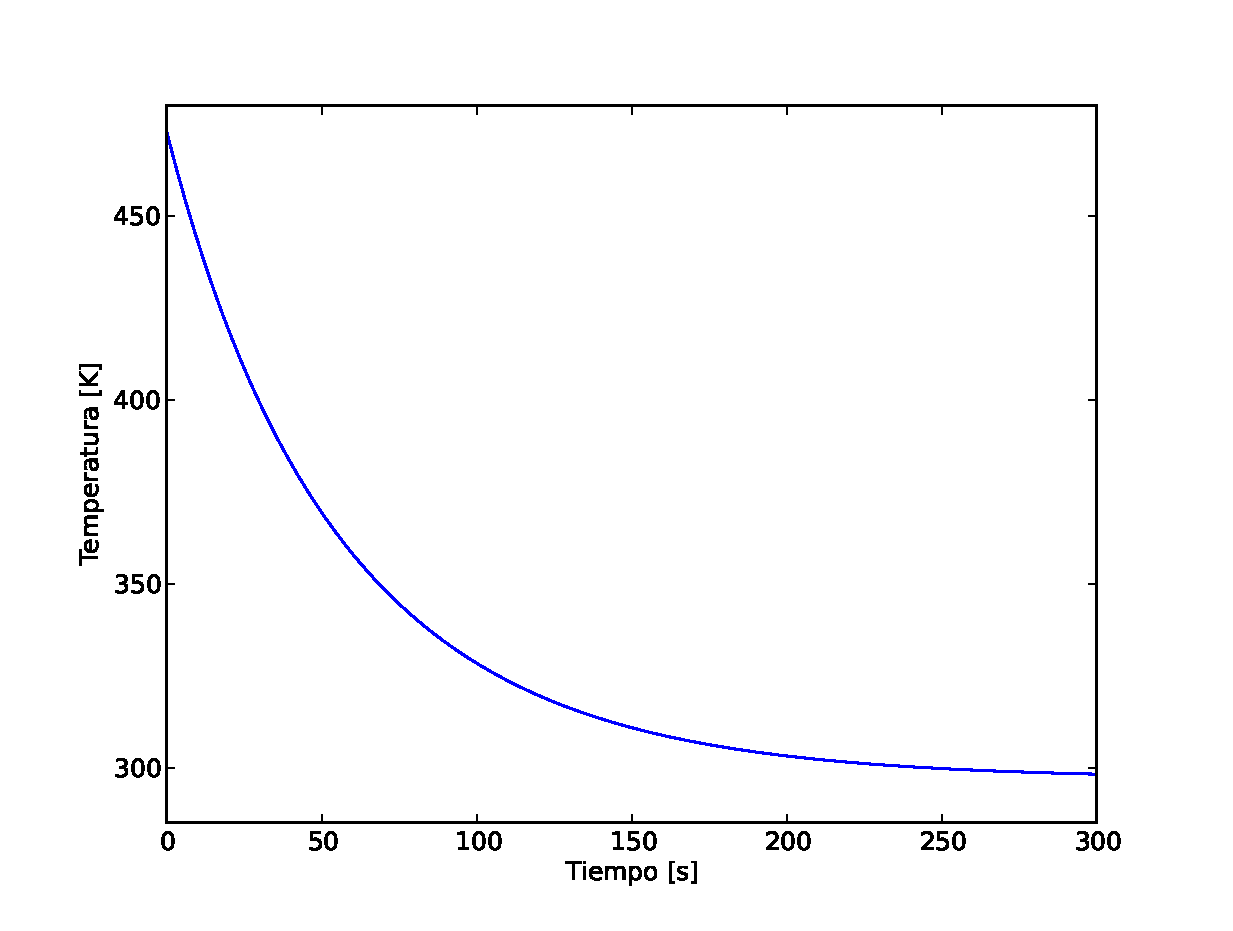
\includegraphics[scale=0.45]{RK4TemperaturaBarra02.eps} 
\end{figure}
\end{frame}
\begin{frame}
\frametitle{Ejercicio a cuenta de examen}
Con la misma pieza met\'{a}lica del ejercicio anterior, ahora consideremos que la T inicial es de $25^{\circ}$ y se calienta internamente de forma el\'{e}ctrica a raz\'{o}n de $q=3000$ W. La ecuaci\'{o}n de temperatura es:
\[ \begin{split}
\dfrac{dT}{dt} =& \dfrac{1}{\rho c v} \left[ q - \epsilon \sigma A \left( T^{4} - 298^{4} \right) - h_{c} A \left( T - 298 \right) \right], \\
 T(0) =& 298
 \end{split} \]
Calcular la temperatura de la pieza hasta \textit{t} = minutos, usando RK4, con $h=0.1$ minutos.
\end{frame}
\end{document}